\documentclass[a4paper,12pt]{article} 
\usepackage{geometry}
\geometry{
	a4paper,
	total={170mm,257mm},
	left=20mm,
	top=20mm,
}
\usepackage{titlesec}
\usepackage{wrapfig}
\titlelabel{\thetitle.\quad} %точка в section

%%% Работа с русским языком
\usepackage{cmap}                    % поиск в PDF
\usepackage{mathtext} 			 	 % русские буквы в формулах
\usepackage[T2A]{fontenc}            % кодировка
\usepackage[utf8]{inputenc}          % кодировка исходного текста
\usepackage[english,russian]{babel}  % локализация и переносы

%Математика
\usepackage{amsmath,amsfonts,amssymb,amsthm,mathtools} % AMS
\usepackage{icomma} % "Умная" запятая

%% Шрифты
\usepackage{euscript}	 % Шрифт Евклид
\usepackage{mathrsfs} % Красивый матшрифт

%% Команды
\DeclareMathOperator{\const}{\mathop{const}}

%% Перенос знаков в формулах
\newcommand*{\hm}[1]{#1\nobreak\discretionary{}
	{\hbox{$\mathsurround=0pt #1$}}{}}

%%% Заголовок
\author{Лазарь Влад Б01-202\\Шептяков Артём Б01-203
		}
\title{\textbf{Измерение удельной теплоёмкости воздуха при постоянном давлении}}
\date{\today}

\begin{document}
	
	\Large \maketitle
	
	\newpage
	
	\section{Введение}
	
	\textbf{Цель работы:} измерить повышение температуры воздуха в зависимости от мощности подводимого тепла и расхода при стационарном течении через трубу; исключив тепловые потери, по результатам измерений определить теплоёмкость воздуха при постоянном давлении.\\\\
	\textbf{В работе используются:} теплоизолированная стеклянная трубка; электронагреватель; источник питания постоянного тока; амперметр, вольтметр (цифровые мультиметры); термопара, подключенная к микровольтметру; компрессор; газовый счётчик;
	секундомер.
	
	\subsection {Теоритическая справка}
	
	Измерение теплоёмкости тел обычно производится в калориметрах, т.е. в сосудах, обеспечивающих теплоизоляцию исследуемого тела от внешней среды. При этом регистрируется изменение его температуры $dT$ в зависимости от количества тепла $\delta Q$, полученного телом от некоторого нагревательного элемента внутри калориметра. Теплоёмкость тела в некотором процессе определяется как их отношение:
	
	\begin{equation*}
		C = \frac{\delta Q}{dT}
		\eqno(1)
	\end{equation*}

	Надёжность измерения определяется, в основном, качеством калориметра. Необходимо, чтобы количество тепла, затрачиваемое на нагревание исследуемого тела, существенно превосходило тепло, расходуемое на нагревание самого калориметра, а также на потери тепла из установки. При измерении теплоёмкости газов эти требования выполнить довольно трудно --- масса газа в калориметре и, следовательно, количество тепла, идущее на его нагревание, как правило, малы. Для увеличения количества нагреваемого газа при неизменных размерах установки в нашей работе исследуемый газ (воздух) продувается через калориметр, внутри которого установлен нагреватель. При этом измеряются мощность нагревателя, масса воздуха, протекающего в единицу времени (расход), и приращение его температуры.
	
	\begin{figure}[h!]
		\centering{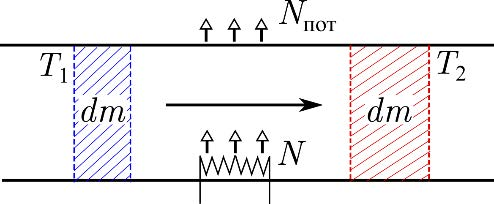
\includegraphics[width=0.4\textwidth]{pictures/pic1.jpg}}
		\caption[]{\label{fig:1} Нагрев газа при течении по трубе}
	\end{figure}

	Рассмотрим газ, протекающий стационарно слева направо через трубу постоянного сечения, в которой установлен нагревательный элемент (см. рис.1). Пусть за некоторое время $dt$ через калориметр прошла малая порция газа массой $dm = q dt$, где\\ $q\ [\frac{кг}{с}]$ -- массовый расход газа в трубе (в расчётах для удобства будем использовать $q\ [\frac{л}{с}]$). Если мощность нагрева равна $N$, мощность тепловых потерь на обмен с окружающей средой $N_{\text{пот}}$, то порция получила тепло $\delta Q =(N - N_{\text{пот}})dt$. С другой стороны, по определению теплоёмкости (1): $\delta Q =c dm \Delta T$ , где $\Delta T = T_2 - T_1$ -- приращение температуры газа, и $c$ — удельная (на единицу массы) теплоёмкость газа в рассматриваемом процессе. При малых расходах газа и достаточно большом диаметре трубы перепад давления на её концах мал, поэтому можно принять, что $P_1 \approx P_2 = P_0$, где $P_0$ - атмосферное давление. Следовательно, в условиях опыта измеряется удельная теплоёмкость при постоянном давлении $C_P$. Таким образом, получаем
	
	\begin{equation}
		\begin{aligned}
			C_p = \dfrac{N - N_{\text{пот}}}{q \Delta T} 
		\end{aligned}
	\end{equation}

	В общем случае давление
	на входе может заметно превышать таковое на выходе
	(например, если труба достаточно узкая и длинная). Рассмотрим течение газа более
	детально, чтобы выяснить пределы применимости $P = const$. Обозначим индексом 1 параметры газа на входе в трубку, индексом 2 --- на выходе из неё. Рассмотрим область, мысленно ограниченную двумя неподвижными плоскостями слева и справа от нагревателя и применим к ней закон сохранения энергии.
	
	\begin{figure}[h!]
		\centering{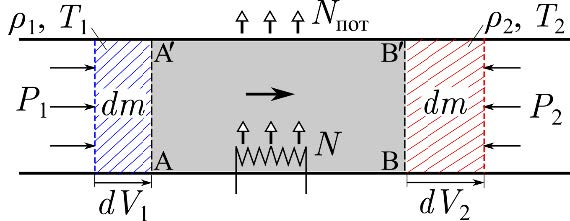
\includegraphics[width=0.5\textwidth]{pictures/pic2.jpg}}
		\caption[]{\label{fig:2} Нагрев газа при течении по трубе}
	\end{figure}
	
	Пусть за время $dt$ газ сместился слева направо на малое расстояние вдоль
	трубки, такое что через левую границу прошёл газ объёмом $dV_1$, а через правую --- $dV_2$. В силу закона сохранения массы имеем
	\[
	m = \rho_1 dV_1 = \rho_2 d V_2,
	\]
	где $dm = q dt$ --- масса газа, прошедшего через некоторое сечение трубки.
	Изменение внутренней энергия газа в рассматриваемой области за счёт переноса вещества составило $dU = (u_2 - u_1)dm$, где $u_{1, 2}$ --- удельные внутренние энергии. Внешние силы совершили работу по перемещению газа $\partial A = P_1 dV_1 - P_2 dV_2$, или с учётом предыдущей формулы:
	\[
	\partial A = - (\frac{P_2}{\rho_2} - \frac{P_1}{\rho_1})dm.
	\]
 
	Учтём также изменение кинетической энергии течения газа, равное $dK = \frac{1}{2}(v_2^2 - v_1^2)dm$, где $v_{1, 2}$ --- скорости течения. Наконец, пусть $\partial Q$ --- количество тепла, суммарно полученное газом в рассматриваемой области --- включая тепло от нагревателя, теплопередачу через стенки и торцы, тепловыделение при трении и т. д. В стационарном состоянии энергия газа, заполняющего калориметр, неизменна, поэтому
	\[
	dU - dA + dK = \partial Q
	\]
	Полученное удобно записать в виде
	\[
	(i_2 - i_1 + \frac{v_2^2}{2} - \frac{v_1^2}{2}) dm = \partial Q,
	\]
	где $i = u + \frac{P}{\rho}$ --- удельная энтальпия газа.
	Это соотношение справедливо для любой стационарно текущей непрерывной среды и представляет собой обобщение известного уравнения Бернулли, учитывающее выделение и потери тепла. Оно справедливо при условии, что в системе устанавливается не только стационарное течение, но и стационарное распределение температуры. Последнее весьма важно для нашего опыта, поскольку время установления может быть довольно велико.
	
	Если предположить, что кинетическая энергия течения мала по сравнени. с энергией нагрева ($dK \ll \partial Q$), то получим 
	\[
	(i_2 - i_1) dm = \partial Q,
	\]
	то есть полученное газом тепло идёт на приращение его энтальпии.
	
	В условмях опыта газ с хорошей точностью можно считать идеальным: $\frac{P}{\rho} = \frac{RT} {mu}$, а теплоёмкость $c_p$ (или $c_v$) не зависящей от температуры. Тогда энальпия (и внутренняя энергия) газа зависит только от температуры и равна $\Delta i = c_p \Delta T$ (т. к. $\Delta u = c_V \Delta T$ и $c_p = c_V + \frac{R}{\mu}$). В таком случае, в этой лабораторной работе мы измеряем удельную теплоёмость газа при постоянном давлении.
	
	
	
	\subsection{Экспериментальная установка:}

 
	Схема установки изображена на рис. 3. Воздух, нагнетаемый компрессором, прокачивается через калориметр. Калориметр представляет собой стеклянную цилиндрическую трубку с двойными стенками, запаянными с торцов.
	
	\begin{figure}[h!]
		\centering{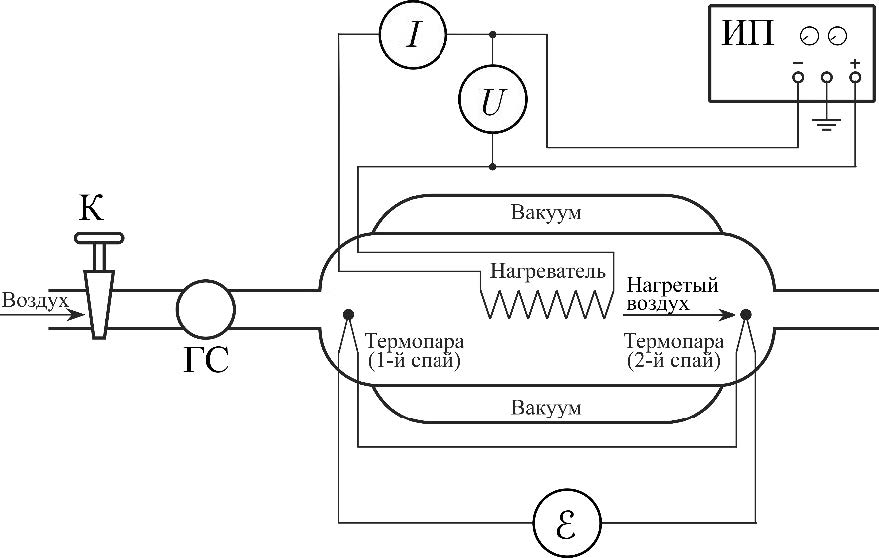
\includegraphics[width=0.8\textwidth]{pictures/pic3.jpg}}
		\caption[]{\label{fig:3} Схема экспериментальной установки}
	\end{figure}
	
	
	Нагреватель в виде намотанной на пенопласт нихромовой проволоки расположен внутри калориметра непосредственно в воздушном потоке. Нагрев проволоки производится от регулируемого источника постоянного тока (ИП).
	Напряжение $U$ на нагревателе и ток $I$ через него регистрируются цифровыми мультиметрами. Таким образом, мощность нагрева равна
	\begin{equation*}
		N = UI
		\eqno(3)
	\end{equation*}
	
	Для измерения разности температур $\Delta T$ служит\\ медно-константановая
	термопара. Один спай термопары расположен в струе воздуха, входящего в
	калориметр, и находится при комнатной температуре, а второй — в струе выходящего нагретого воздуха. Константановая проволока термопары расположена внутри калориметра, а медные проводники подключены к цифровому вольтметру. Возникающая в термопаре ЭДС $\varepsilon$ пропорциональна разности температур $\Delta T$ спаев: 
	\begin{equation*}
		\varepsilon =\beta \Delta T
		\eqno(4)
	\end{equation*}
	
	где $\beta = 40.7\ \frac{мкВ}{К}$ — чувствительность медно-константановой термопары в рабочем диапазоне температур (20$^\circ C$–- 30$^\circ C$ ). ЭДС регистрируется с помощью микровольтметра.
	
	Объём воздуха, прошедшего через калориметр, измеряется газовым счётчиком ГС. Для регулировки расхода служит кран К. Время $\Delta t$ прохождения
	некоторого объема $\Delta V$ воздуха измеряется секундомером. Объёмный расход равен $\frac{\Delta V}{\Delta t} $, массовый расход может быть найден как 
	\begin{equation*}
		q = \rho_{0} \frac{\Delta V}{\Delta t}
		\eqno(5)
	\end{equation*}
	
	где $\rho_{0}$ — плотность воздуха при комнатной температуре, которая в свою очередь может быть получена из уравнения Менделеева–Клапейрона: $\rho_{0}= \frac{\mu P_{0} }{R T_{0}},$ где $P_{0}$ — атмосферное давление, $T_{0}$ — комнатная температура (в Кельвинах), $\mu = 29,0$ г/моль --- средняя молярная масса (сухого) воздуха.
	
	Учитывая особенности устройства калориметра, следует ожидать, что мощность нагревателя расходуется не только на нагрев массы прокачиваемого воздуха, но и частично теряется за счет нагрева внутренних стенок термостата и рассеяния тепла через торцы термостата. Можно предположить, что при небольшом нагреве ($\Delta T \ll T_{0}$) мощность потерь тепла $N_{пот}$ прямо пропорциональна разности температур:
	\begin{equation*}
		N_{пот} = \alpha \Delta T
		\eqno(6)
	\end{equation*}
	
	где $\alpha$ — некоторая константа. При этом условии основное соотношение (2) принимает вид 
	\begin{equation*}
		N = (C_{P}q +\alpha)\Delta T
		\eqno(7)
	\end{equation*}
	
	Следовательно, при фиксированном расходе воздуха ($q = \const$) подводимая мощность и разность температур связаны прямой пропорциональностью ($N(\Delta T)$ -- линейная функция).
	
	\begin{figure}[h!]
		\centering{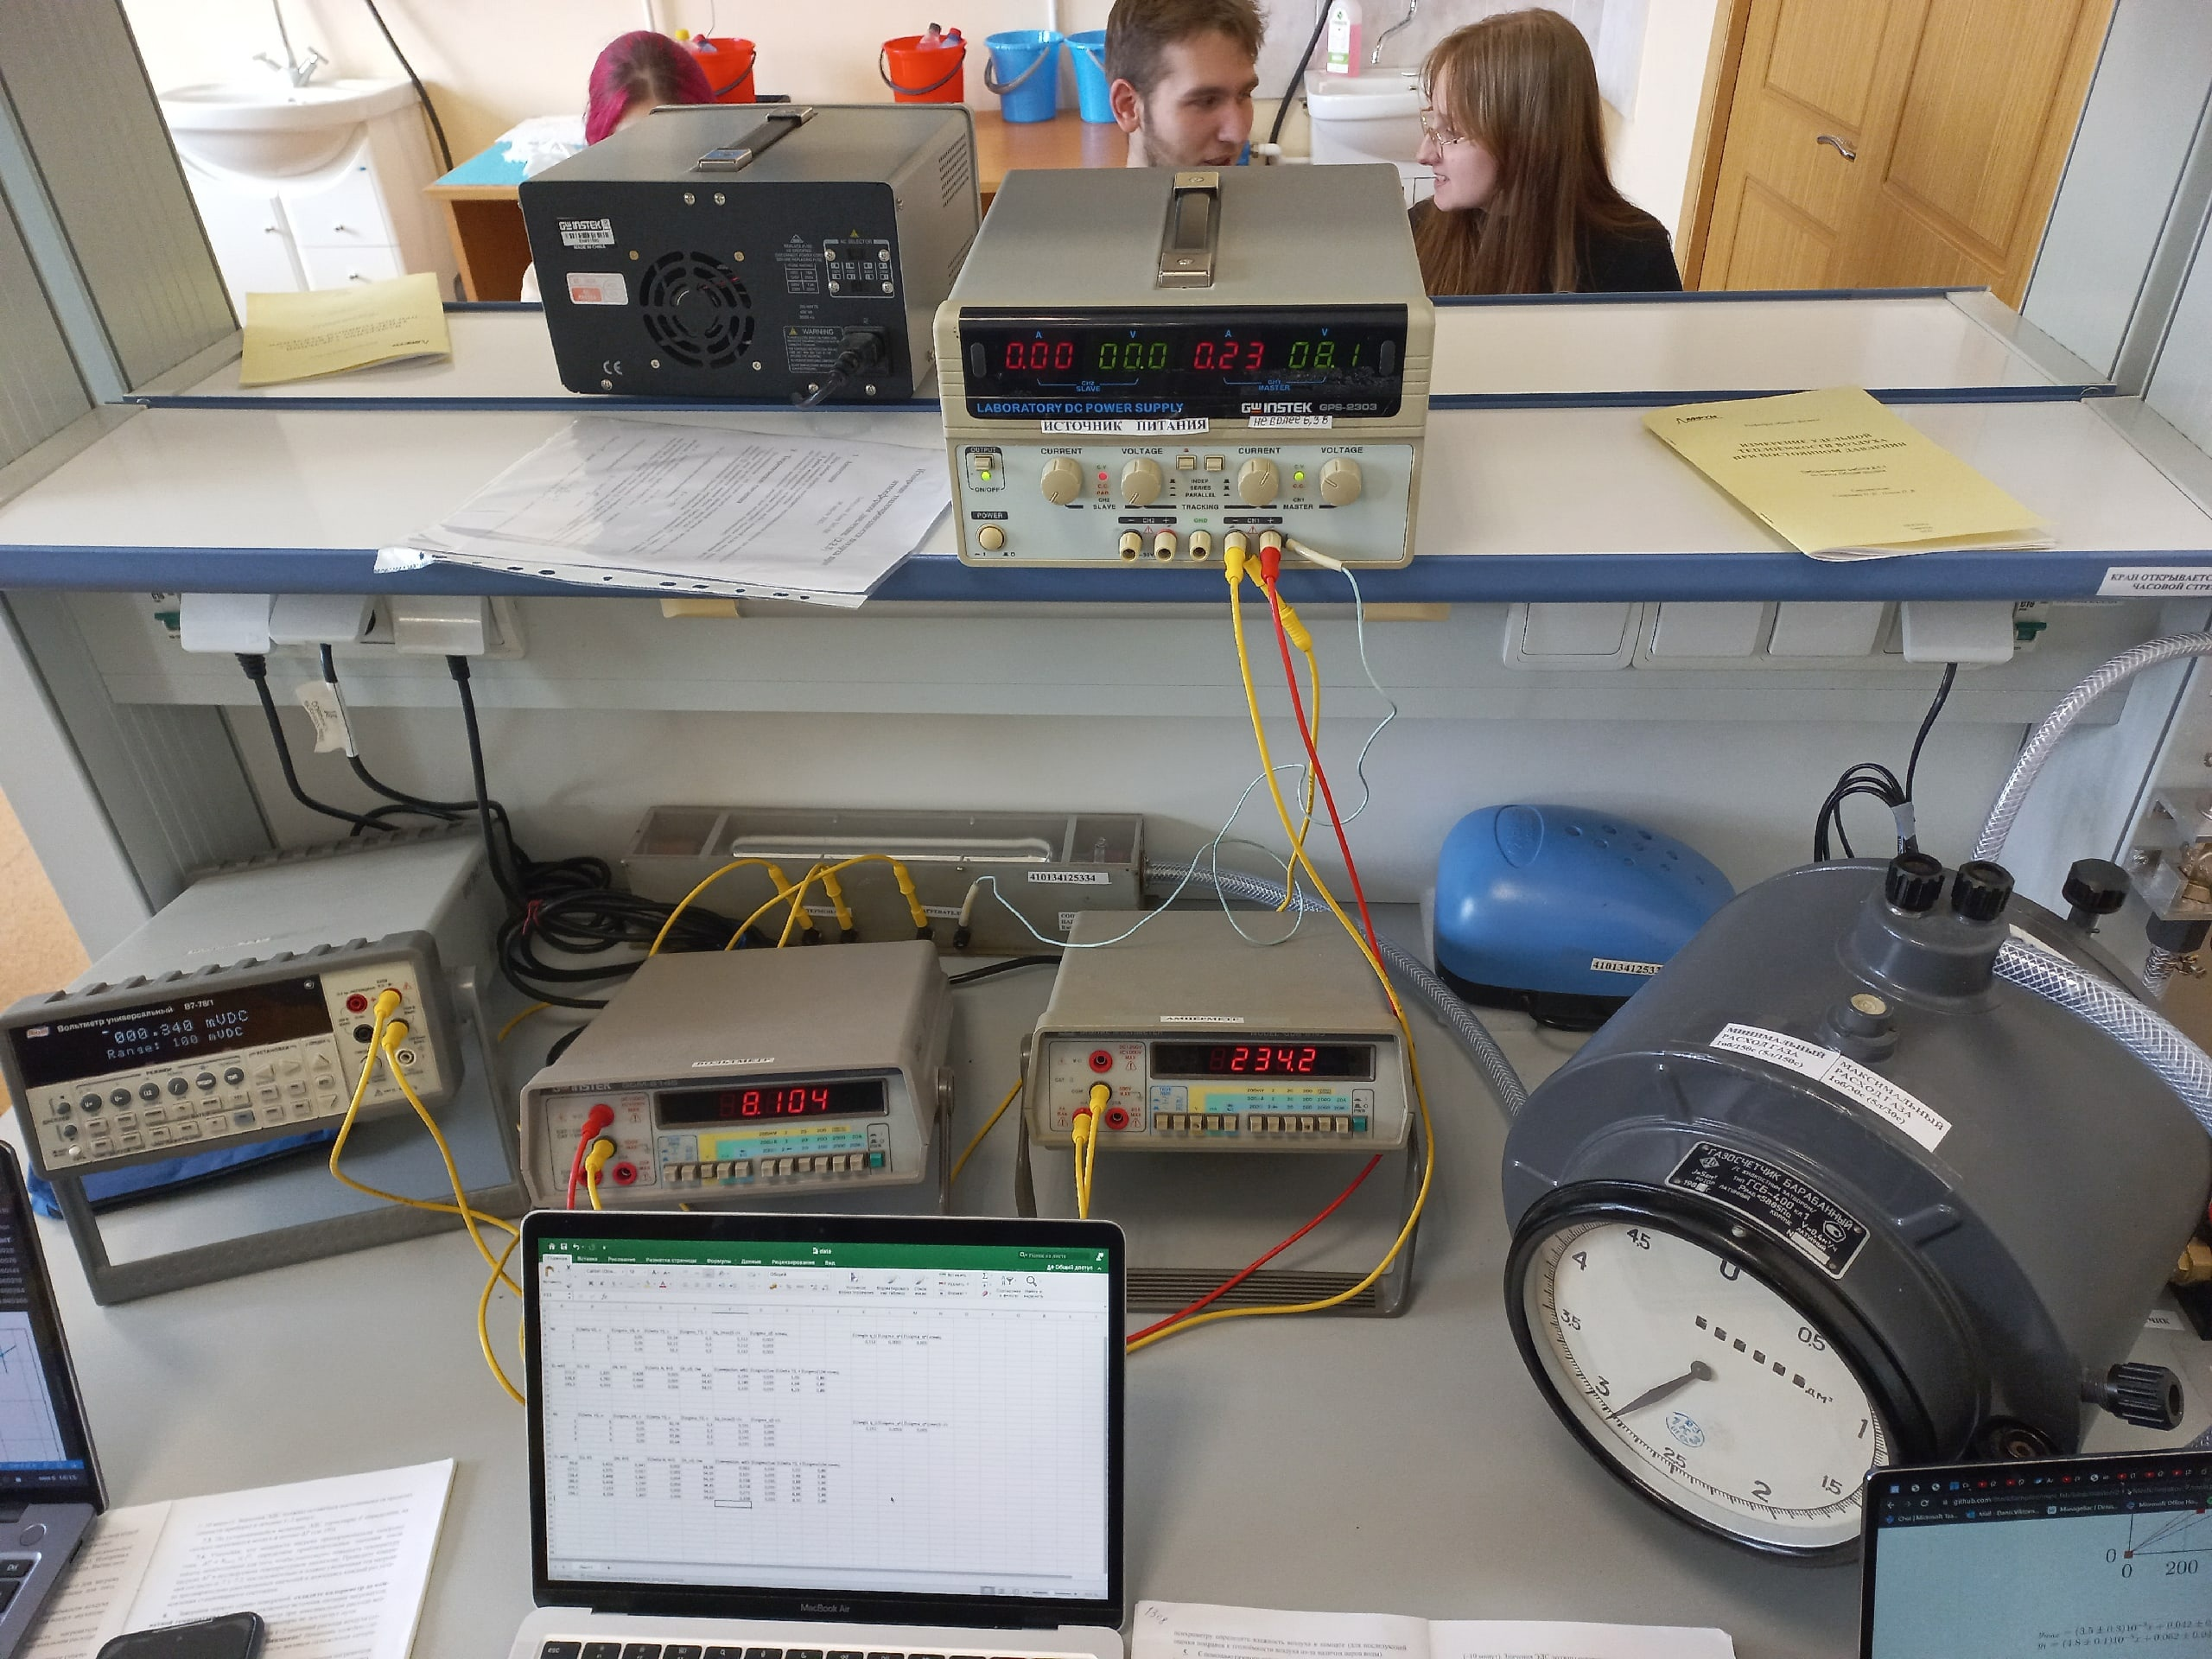
\includegraphics[width=0.7\textwidth]{pictures/ust3.jpg}}
		\caption[]{\label{fig:4} Фото экспериментальной установки}
	\end{figure}

	\begin{figure}[h!]
		\centering{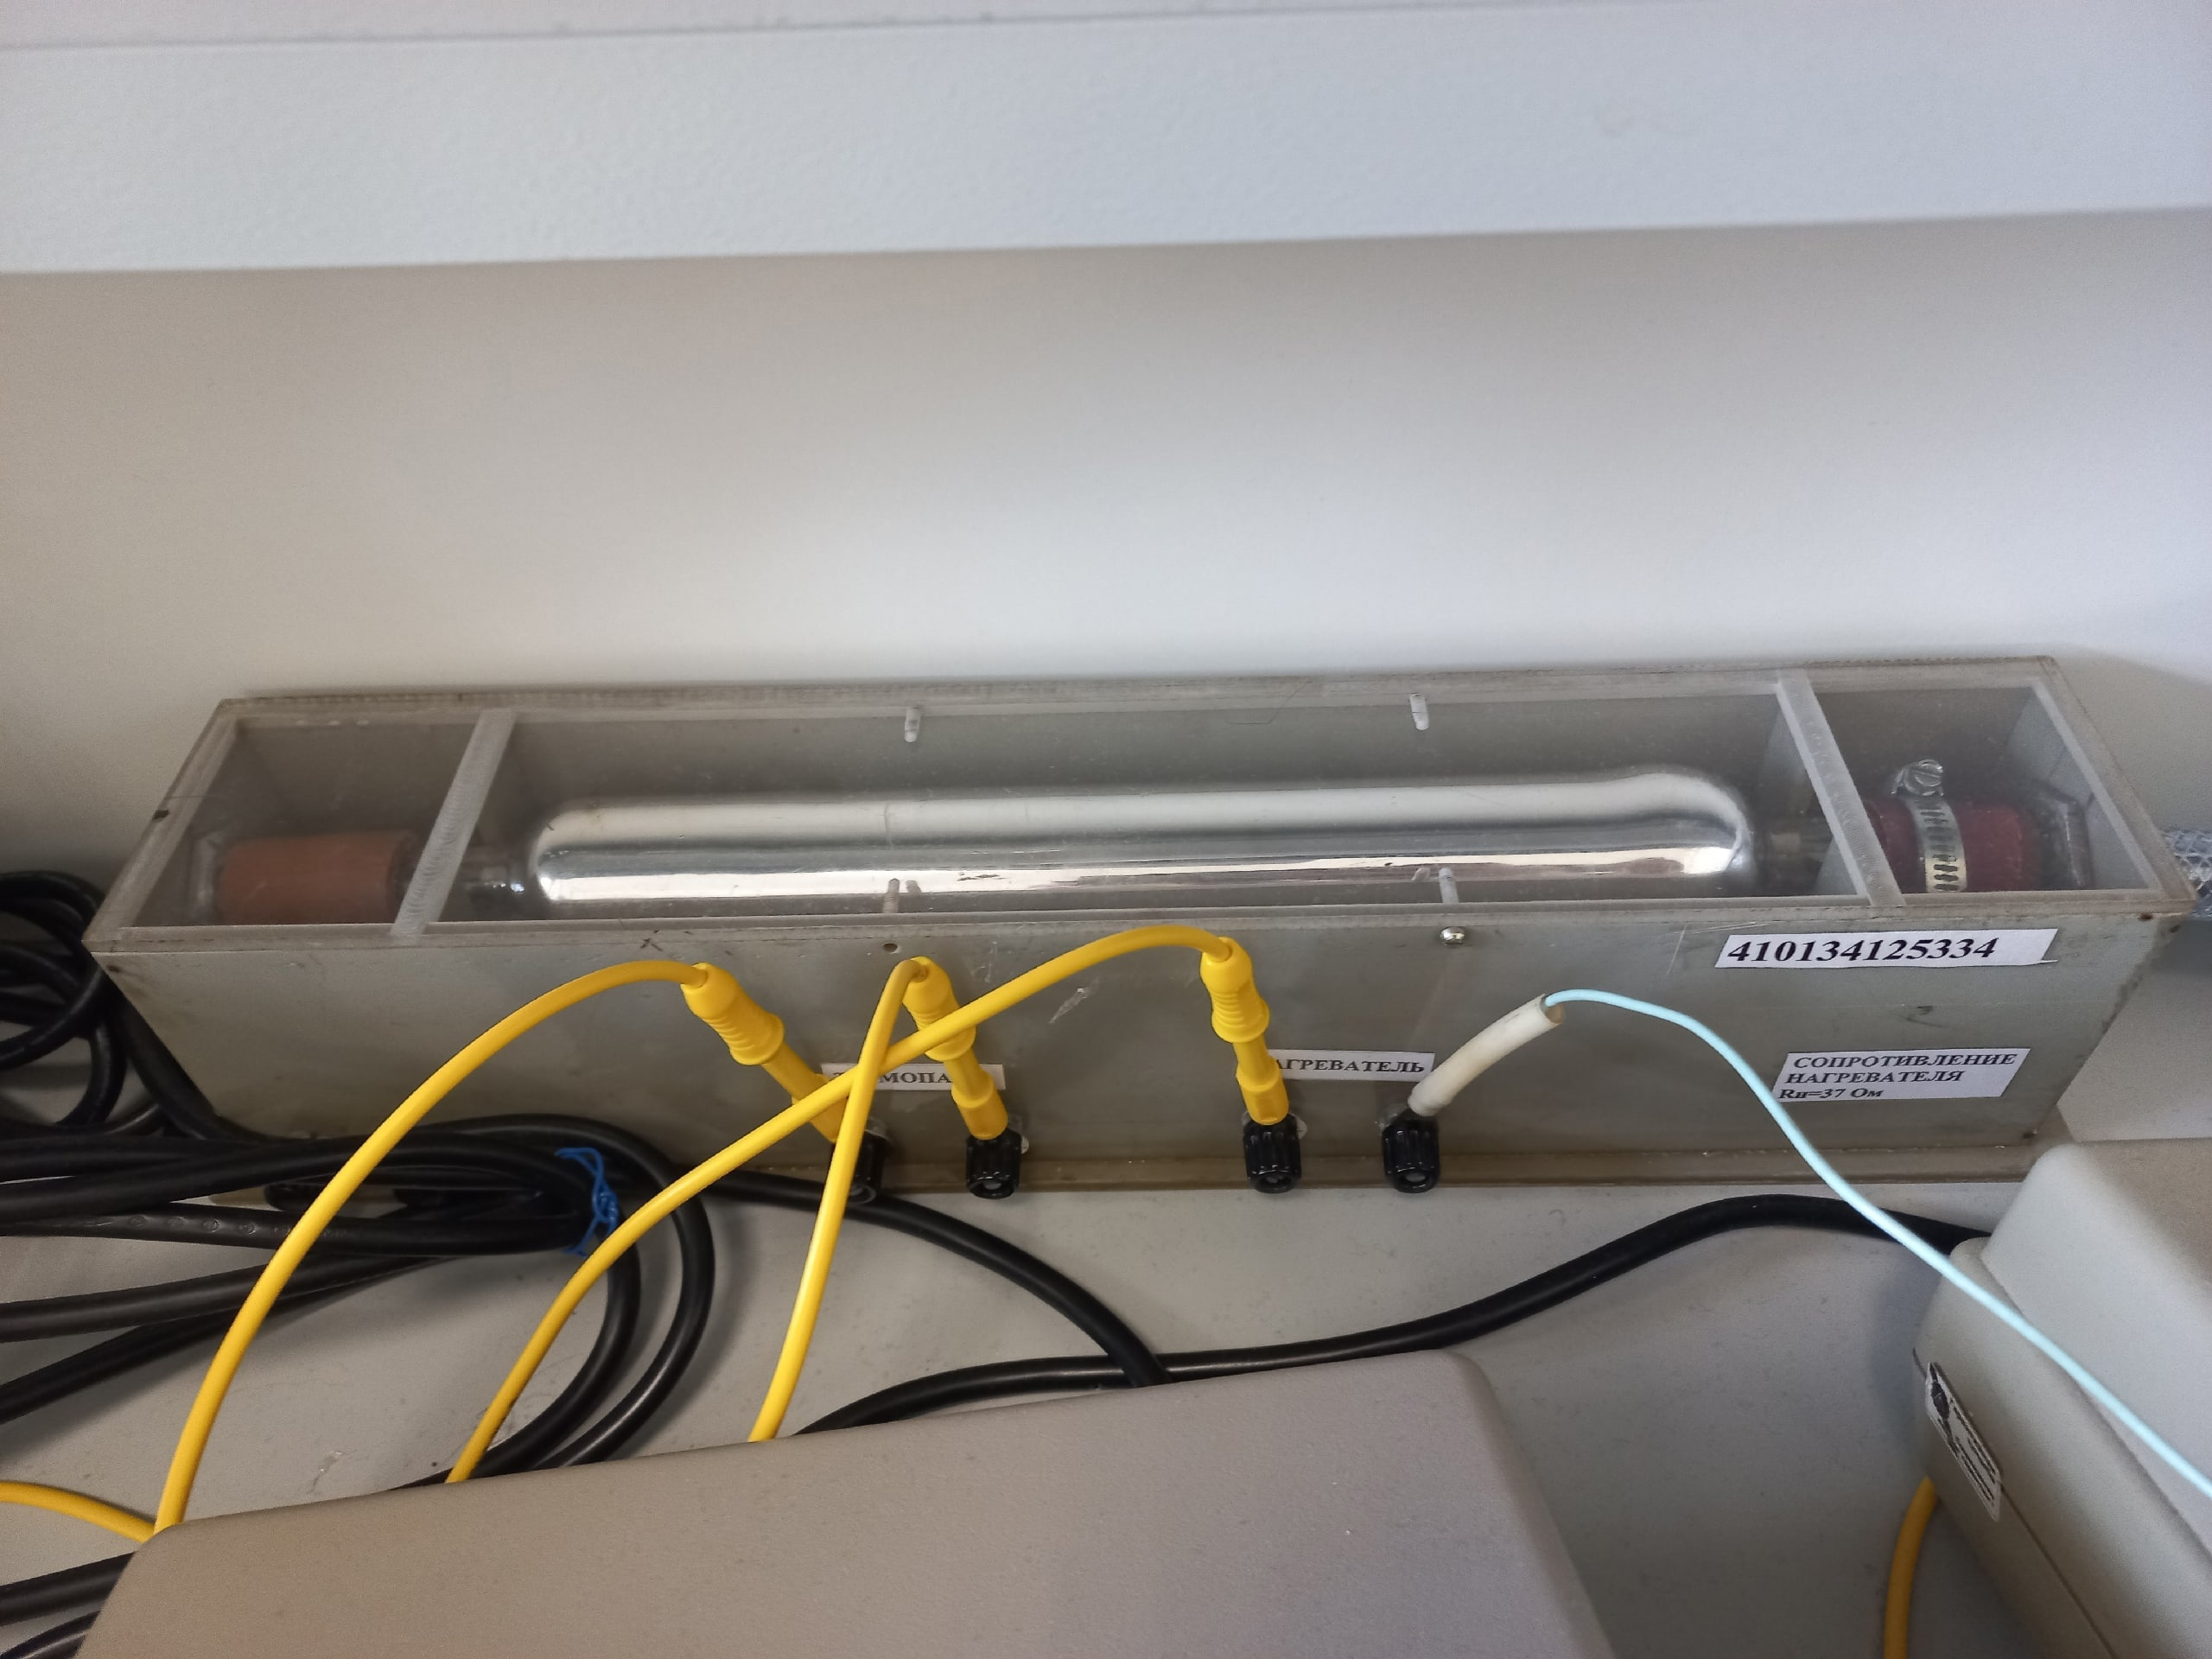
\includegraphics[width=0.7\textwidth]{pictures/ust1.jpg}}
		\caption[]{\label{fig:5} Фото калориметра}
	\end{figure}
	
	\newpage
	\newpage
	
	\section*{Ход работы}
	\subsection*{Подготовка к эксперименту}
	\begin{enumerate}
		\item [\textbf{1.}] Подготовим к работе газовый счетчик: проверим, заполнен ли он водой, установим счетчик по уровню.
		\item [\textbf{2.}] Начинать измерения следует при условии, что калориметр охлажден до комнатной температуры. Для охлаждения включим компрессор и, открывая кран К, установим максимально возможный расход воздуха. Источник постоянного тока при этом выключен. Для проверки корректности работы газового счетчика стоит убедиться, что при постоянном расходе его стрелка вращается равномерно.
		\item [\textbf{3.}] Включим вольтметр, предназначенный для измерения ЭДС термопары. Если показания вольтметра отличны от нуля, продуем калориметр воздухом до полного охлаждения калориметра (т.е. до установления нуля на цифровом дисплее вольтметра).
		\item [\textbf{4.}]Запишем значения температуры, давления и влажности в комнате, необходимые для расчета расхода прокачиваемого воздуха.
		\begin{center}
			\begin{tabular}{|c|c|c|}
				\hline
				& Значение & $\sigma$ \\ \hline
				$P$, Па    & 99970   & 1        \\ \hline
				$T$, К     & 294,8   & 0,1      \\ \hline
				$\varphi$  & 35,9\%  & 1\%      \\ \hline
			\end{tabular}
		\end{center}
		\item [\textbf{5.}] С помощью газового счетчика и секундомера измерим максимальный расход воздуха $\frac{\Delta V}{\Delta t}$ $\left[\frac{л}{с}\right]$. Измерения проведем несколько раз и определим среднее значение расхода.
		\begin{center}
			\begin{tabular}{|c|c|c|c|c|c|c|}\hline
                $\rho$, $кг/м^3$ & $\sigma_{\rho}$, $кг/м^3$ & $C_p^{\text{th}}$, $\dfrac{Дж}{кг \cdot K}$ & $\sigma_V$, л & $\sigma_t$, c  & $\sigma_t$, c & $\sigma_t$, с \\\hline
                1,1502 & 0,0005 & 1005  & 0,02   & 0,20  & 0,01 & 0,20\\\hline
                \end{tabular}
			
			\begin{tabular}{|c|c|c|c|}
				\hline
				\multicolumn{4}{|c|}{\text{Измерение расхода $q_1$}} \\
				\hline
				$\Delta V$, л & $\Delta t, c$ & $q$, л/с  & $\sigma_q$, л/с \\ \hline
				5             & 30,47         & 0,1641    & 0,0013          \\ \hline
				5             & 30,81         & 0,1623    & 0,0012	 	    \\\hline
				5             & 30,69         & 0,1629    & 0,0012          \\ \hline
				5             & 30,75         & 0,1626    & 0,0012          \\ \hline
				5             & 30,81         & 0,1623    & 0,0012          \\ \hline
				5             & 30,84         & 0,1621    & 0,0012          \\ \hline
				5             & 30,65         & 0,1631    & 0,0012          \\ \hline
				5             & 30,72         & 0,1628    & 0,0012          \\ \hline
			\end{tabular}
			     \\ \phantom{Русичи} \\
			\begin{tabular}{|c|c|c|c|}
				\hline
				\multicolumn{4}{|c|}{\text{Измерение расхода $q_2$}} \\
				\hline
				$\Delta V$, л & $\Delta t, c$ & $q$, л/с  & $\sigma_q$, л/с \\ \hline
				5             & 50,87         & 0,0983    & 0,0006          \\ \hline
				5             & 50,84         & 0,0983    & 0,0006	 	    \\\hline
				5             & 50,75         & 0,0985    & 0,0006          \\ \hline
				5             & 50,84         & 0,0983    & 0,0006          \\ \hline
				5             & 50,85         & 0,0983    & 0,0006          \\ \hline
				5             & 50,81         & 0,0984    & 0,0006          \\ \hline
				5             & 50,69         & 0,0986    & 0,0006          \\ \hline
				5             & 50,75         & 0,0985    & 0,0006          \\ \hline
			\end{tabular}
                \\ \phantom{Ящеры} \\
			\begin{tabular}{|c|c|c|c|}
				\hline
				\multicolumn{4}{|c|}{\text{Измерение расхода $q_3$}} \\
				\hline
				$\Delta V$, л & $\Delta t, c$ & $q$, л/с  & $\sigma_q$, л/с \\ \hline
				5             & 71,53         & 0,0699    & 0,0003          \\ \hline
				5             & 71,34         & 0,0701    & 0,0003	 	    \\\hline
				5             & 71,38         & 0,0700    & 0,0003          \\ \hline
				5             & 71,56         & 0,0699    & 0,0003          \\ \hline
				5             & 71,62         & 0,0698    & 0,0003          \\ \hline
				5             & 71,88         & 0,0696    & 0,0003          \\ \hline
				5             & 71,84         & 0,0696    & 0,0003          \\ \hline
				5             & 71,62         & 0,0698    & 0,0003          \\ \hline
			\end{tabular}
		\end{center}
	\end{enumerate}
	\subsection*{Проведение измерений}
	\begin{enumerate}
        \item [\textbf{6.}] Оцениваем величину тока нагревателя $I_0$, требуемого для нагрева воздуха на $\Delta T = 2\ К$. Для этого определяем теоретическое значение удельной теплоёмкости воздуха при постоянном давлении $C_p^{th}$ [ $ \frac{Дж}{кг}\cdot$К ], считая воздух смесью двухатомных идеальных газов; оцениваем минимальную мощность\\ $N_0 \approx 0,326$ Вт ($N \geq C_p^{th} q \Delta T$), необходимую для нагрева газа при максимальном расходе $q_{max}$ на $\Delta T_0 = 2\ К$; учитывая, что сопротивление проволоки нагревателя составляет приблизительно $R_H \approx 35$ Ом и в процессе опыта практически не меняется, определияем искомое значение тока $$I_0 = \sqrt{\dfrac{N_0}{R_H}} \approx 93 \text{ mA}. $$
        
    \item [\textbf{7.}]Проведём измерение зависимости разности температур от мощности нагрева $N(\Delta T)$ при максимальном расходе воздуха $q_1 = q_{max}$. Причём рекомендуется измерить 4--5 точек в диапазоне температур (измерим 6 точек для надёжности) $N(\Delta T)$\ от $\approx 2K$ до $\approx 10K$.
    \begin{enumerate}
    \item [\textbf{7.1}] Чтобы начать нагрев, включаем источник питания (ИП) нагревателя и устанавливаем на нём такое напряжение, чтобы ток через нить нагревателя составлял\\ $I_1 \sim 2\div2,5\ I_0$ (см. п. 6). Записываем значения тока $I$ и напряжения $U$ в цепи. Рассчитаем мощность $N$ нагрева, а также сопротивление нити нагревателя $R_{\text{н}}$.
    \item [\textbf{7.2}] После включения нагрева (или после изменения его мощности) дожидаемся установления стационарного состояния системы. Первоначальный прогрев калориметра происходит достаточно долго ($\sim$ 20 минут). Значения ЭДС $\varepsilon$ вольтметра, подключенного к термопаре, должны оставаться постоянными (в пределах точности прибора) в течение 2---3 минут.
    \item [\textbf{7.3}] По величине $\varepsilon$ определим значение $\Delta T$ (см. (4)). Учитывая, что $\Delta T \varpropto N \varpropto I^2$, определяем значения токов накала, необходимые для того, чтобы равномерно повышать температуру нагрева $\Delta T$ до требуемого значения. Проводим измерения согласно п. 7.1---7.2, последовательно увеличивая ток нагрева до расчётных значений.
    \end{enumerate}
		\begin{center}
	
			
			\begin{tabular}{|c|c|c|c|c|c|c|}
				\hline
				\multicolumn{7}{|c|}{$q_1 = (0,1628 \pm 0,0012)$, л/c} \\ \hline
				$I$, мА 			& 99,6 		& 127,2 	& 158,3  	& 186,6  & 209,5  	& 234,1  \\ \hline
				$U$, В 				& 3,425	 	& 4,375 	& 5,448  	& 6,428  & 7,232  	& 8,104  \\ \hline
				$N$, Вт 			& 0,3411	& 0,5565 	& 0,8624 	& 1,1995 & 1,5151 	& 1,8971 \\ \hline
				$\varepsilon$, мкВ 	& 63 		& 102		& 158 		& 217 	 & 272 		& 338 	 \\ \hline
				$\Delta T, K$ 		& 1,548 	& 2,506		& 3,882	 	& 5,332  & 6,683	& 8,305  \\ \hline
				$R$, Ом 			& 34,39 	& 34,39		& 34,42	 	& 34,45  & 34,52 	& 34,62	 \\ \hline
				$\sigma_I$, мА 				& 0,01 	 & 0,01   	& 0,01 		& 0,01	 & 0,01		& 0,01	\\ \hline
				$\sigma_U$, В 				& 0,001  & 0,001  	& 0,001 	& 0,001  & 0,001 	& 0,001 \\ \hline
				$\sigma_N$, Вт 				& 0,0001 & 0,0001 	& 0,0002 	& 0,0002 & 0,0002 	& 0,0003 \\ \hline
				$\sigma_\varepsilon$, мкВ 	& 1 	 & 1 	  	& 1 		& 1 	 & 1 		& 1\\ \hline
				$\sigma_{\Delta T}, K$ 		& 0,025	 & 0,026	& 0,028 	& 0,031	 & 0,0334	& 0,0374 \\ \hline
				$\sigma_R$, Ом 				& 0,01 	 & 0,01 	& 0,01 		& 0,01	 & 0,01 	& 0,01 \\ \hline
			\end{tabular}
			\\ \phantom{Ящеры} \\
			
			\begin{tabular}{|c|c|c|c|c|c|c|}
				\hline
				\multicolumn{7}{|c|}{$q_2 = (0,0984 \pm 0,0006)$, л/c} \\ \hline
				$I$, мА 			& 71,9 		& 100,1		& 119,7		& 138,3  & 156,9	& 173,6  \\ \hline
				$U$, В 				& 2,474		& 3,444		& 4,121		& 4,762  & 5,404	& 5,985  \\ \hline
				$N$, Вт 			& 0,1779	& 0,3447	& 0,4933	& 0,6586 & 0,8479	& 1,0390 \\ \hline
				$\varepsilon$, мкВ 	& 49 		& 97		& 138 		& 184 	 & 240		& 295 	 \\ \hline
				$\Delta T, K$ 		& 1,204		& 2,383		& 3,391		& 4,521  & 5,897	& 7,248  \\ \hline
				$R$, Ом 			& 34,41 	& 34,41		& 34,43		& 34,43  & 34,44	& 34,48	 \\ \hline
				$\sigma_I$, мА 				& 0,01 	 & 0,01   	& 0,01 		& 0,01	 & 0,01		& 0,01	\\ \hline
				$\sigma_U$, В 				& 0,001  & 0,001  	& 0,001 	& 0,001  & 0,001 	& 0,001 \\ \hline
				$\sigma_N$, Вт 				& 0,0001 & 0,0001 	& 0,0001 	& 0,0002 & 0,0002 	& 0,0002 \\ \hline
				$\sigma_\varepsilon$, мкВ 	& 1 	 & 1 	  	& 1 		& 1 	 & 1 		& 1		\\ \hline
				$\sigma_{\Delta T}, K$ 		& 0,025  & 0,026	& 0,027 	& 0,029	 & 0,032	& 0,035 \\ \hline
				$\sigma_R$, Ом 				& 0,02 	 & 0,01 	& 0,01 		& 0,01	 & 0,01 	& 0,01 \\ \hline
			\end{tabular}
		      \\ \phantom{Русичи} \\
			\begin{tabular}{|c|c|c|c|c|c|c|}
				\hline
				\multicolumn{7}{|c|}{$q_3 = (0,0698 \pm 0,0003)$, л/c} \\ \hline
				$I$, мА 			& 73,5 		& 93,4		& 112,5		& 129,8  & 145,6	& 163,8 \\ \hline
				$U$, В 				& 2,53		& 3,215		& 3,872		& 4,468  & 5,013	& 5,644  \\ \hline
				$N$, Вт 			& 0,1860	& 0,3003	& 0,4356	& 0,5799 & 0,7299	& 0,9245 \\ \hline
				$\varepsilon$, мкВ 	& 68 		& 110		& 161 		& 218 	 & 275		& 351 	 \\ \hline
				$\Delta T, K$ 		& 1,671		& 2,703		& 3,956		& 5,356  & 6,757	& 8,624  \\ \hline
				$R$, Ом 			& 34,42 	& 34,42		& 34,42		& 34,42  & 34,43	& 34,46	 \\ \hline
				$\sigma_I$, мА 				& 0,01 	 & 0,01   	& 0,01 		& 0,01	 & 0,01		& 0,01	\\ \hline
				$\sigma_U$, В 				& 0,001  & 0,001  	& 0,001 	& 0,001  & 0,001 	& 0,001 \\ \hline
				$\sigma_N$, Вт 				& 0,0001 & 0,0001 	& 0,0001 	& 0,0001 & 0,0002 	& 0,0002 \\ \hline
				$\sigma_\varepsilon$, мкВ 	& 1 	 & 1 	  	& 1 		& 1 	 & 1 		& 1		\\ \hline
				$\sigma_{\Delta T}, K$ 		& 0,025  & 0,026	& 0,028		& 0,031	 & 0,034	& 0,038 \\ \hline
				$\sigma_R$, Ом 				& 0,01 	 & 0,01 	& 0,01 		& 0,01	 & 0,01 	& 0,01 \\ \hline
			\end{tabular}

		\end{center}
	\end{enumerate}
	\subsection*{Обработка результатов измерений}
	\begin{enumerate}
		\item [\textbf{8.}] Строим графики зависимости $N(\Delta T)$ для каждого расхода воздуха $q$. Проверяем, выполняется ли предположение о том, что тепловые потери пропорциональные разности температур. Аппроксимируя зависимость прямой $y = kx$, найдём угловые коэффициенты $k_i$ для каждого расхода $q_i$ с помощью метода наименьших квадратов.
		
		\begin{center}
			\begin{figure}[]
				\centering{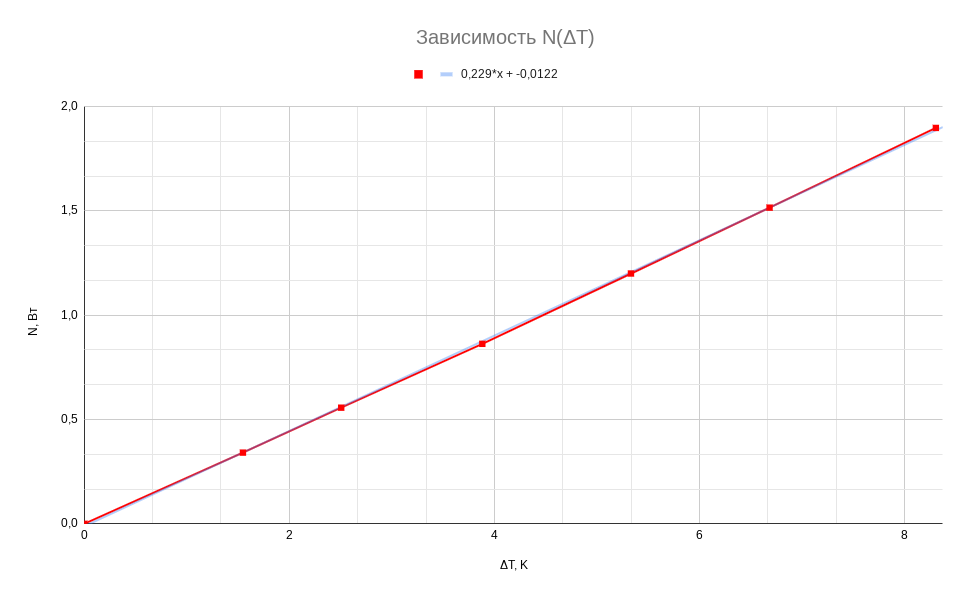
\includegraphics[width=\textwidth]{pictures/1.png}}
				\caption[]{\label{fig:6} график для $q_1$}
			\end{figure}
			\begin{figure}[]
				\centering{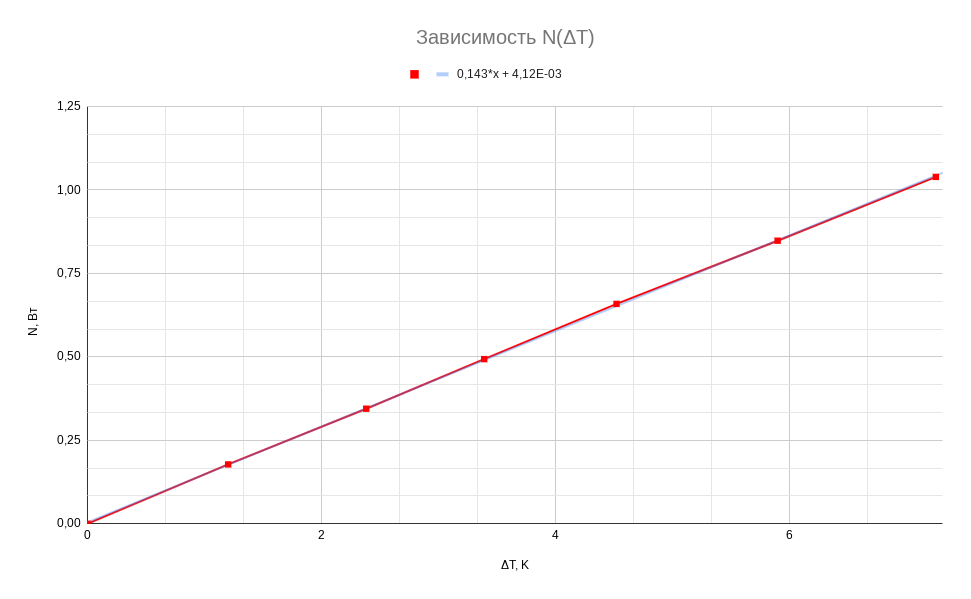
\includegraphics[width=\textwidth]{pictures/2.png}}
				\caption[]{\label{fig:7} график для $q_2$}
			\end{figure}
			\begin{figure}[]
				\centering{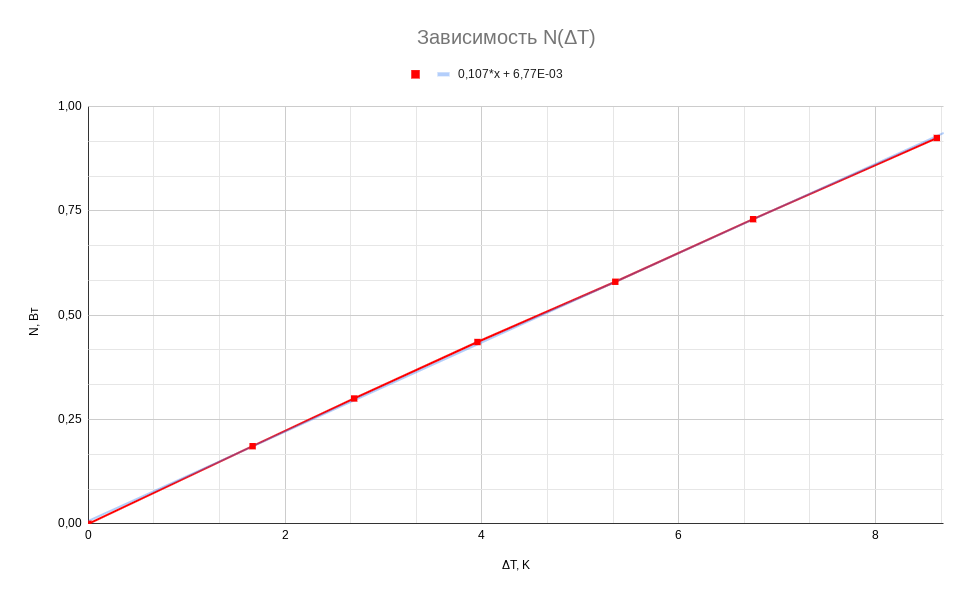
\includegraphics[width=\textwidth]{pictures/3.png}}
				\caption[]{\label{fig:8} график для $q_3$}
			\end{figure}
		\end{center}
		\newpage
  		\newpage
    
		\item [\textbf{9.}] Теперь проанализируем три графика зависимости $N(\Delta T)$ и оценим значения $C_p$ по формуле (7). Получим систему уравнений
            \begin{equation*}
                \begin{cases}
                   0,143 = С_p \cdot 0,0000984 + \alpha\\
                   0,107 = С_p \cdot 0,0000698 + \alpha
                 \end{cases}
                \end{equation*}
            И сразу вернёмся к подсчёту удельной $C_p^{\text{уд}} = \frac{C_p}{\rho}:$
		$$C_p^{\text{уд}} = \frac{k_2 - k_3}{q_2 - q_3} \cdot \frac{1}{\rho} = 1094\ \frac{\text{Дж}}{\text{кг} \cdot\text{К}}$$

            Оценим погрешность по формуле
            \noindent
                \[\sigma_{C_p^{\text{уд}}}^2 =\left(\frac{dC_p}{dk_2}\sigma_{k_2}\right)^2 + \left(\frac{dC_p}{dk_3}\sigma_{k_3}\right)^2 + \left(\frac{dC_p}{dq_2}\sigma_{q_2}\right)^2 + \left(\frac{dC_p}{dq_3}\sigma_{q_3}\right)^2 + \left(\frac{dC_p}{d\rho}\sigma_{\rho}\right)^2 \]
                $$\sigma_{C_p^{\text{уд}}} = C_p^{\text{уд}}\sqrt{\frac{\sigma_{k_2}^2+\sigma_{k_3}^2}{(k_2 - k_3)^2} + \frac{\sigma_{q_2}^2+\sigma_{q_3}^2}{(q_2 - q_3)^2} + \left(\frac{\sigma_\rho}{\rho}\right)^2} = 39\ \frac{\text{Дж}}{\text{кг} \cdot \text{К}}$$

            \begin{center}
		\begin{tabular}{|c|c|c|c|}
			\hline
			$k$, Вт/K & $\sigma_k$, Вт/K & $q$, л/c & $\sigma_q$, г/c \\ \hline
			0,143 & 0,0008 & 0,0984 & 0,0006 \\ \hline
			0,107 & 0,0005 & 0,0698 & 0,0003 \\ \hline
		\end{tabular}
            \end{center}

            Итоге получаем $C_p^{\text{уд}} = (1094 \pm 39)\ \frac{Дж}{кг \cdot K}$.
            \\Для сравнения -- табличная $C_p^{\text{уд}} = 1005\ \frac{\text{Дж}}{кг \cdot K}$.
	
		\item [\textbf{10.}] Оценим величину $N_{\text{пот}} = \alpha \cdot \Delta T$ через коэффициент $\alpha$: 
		$$ \alpha = \frac{q_2 k_3 - q_3 k_2}{q_2 - q_3} \approx 0,006$$
	\end{enumerate}

        \section{Вывод}
        
            В работе были измерены повышение температуры воздуха в зависимости от мощности подводимого тепла и расход при стационарном течении через трубу. По
        результатам измерений были определены теплоёмкость воздуха при постоянном давлении и оценена мощность потерь калориметра.\\
        Не совсем точные результаты могут быть вызваны тем, что охлаждение калориметра занимает много времени, поэтому значения тока, напряжения, ЭДС изменялись значительно. Сильно могли повлиять и изменение влажности воздуха в процессе выполнения работы (с 35,9 \% до 60 \%). Также стоит учитывать, что воздух -- не смесь идеальных двухатомных газов.
\end{document}